\chapter{A Verifiable Gradient Inversion Attack In Federated Learning}

\section{Proof of Proposition \ref{prop:sample_isolation}}
\label{app:proof_prop1}

\begin{proposition}
Consider the non-empty slice delimited at round $t$ by the hyperplanes
$\mathbf w^\top \x+\hat b_k^t=0$ and $\mathbf w^\top \x+\hat b_{k+1}^t=0$,
and suppose that it contains $m\le d$ linearly independent inputs. Assume that
the common first-layer direction $\mathbf w$ is drawn once from a distribution
absolutely continuous with respect to the Lebesgue measure. At each attack round,
assume that the vectorized weights and biases of the layers following the
attacked layer are redrawn independently of the past from absolutely continuous
distributions, supported on parameters for which each downstream hidden layer
has at least two fixed ReLU gates active on all inputs in the slice. Finally,
assume that, for every sample $j$, all level sets of
$\partial \loss_j/\partial z^L$ are Lebesgue-null.

Then, almost surely, the span condition
\[
\slice_k^t
\in
\operatorname{span}\left(
\slice_k^{t+1},\ldots,\slice_{k+q-2}^{t+1}
\right)
\]
implies that every non-empty sub-slice induced at round $t+1$ contains exactly
one input. Hence, when the span condition holds, the original slice contains
as many inputs as there are non-null induced slice vectors, and therefore at
most $q-1$ inputs.
\end{proposition}



\begin{proof}
For each sample $j$, define
\[
\psi_j(z)
:=
\frac{1}{B}\frac{\partial \ell(z,y_j)}{\partial z}.
\]
Every level set $\psi_j^{-1}(c)$ has one-dimensional Lebesgue
measure zero.
Let $\mathcal X$ denote the non-empty slice delimited at round $t$ by the hyperplanes
$\mathbf w \x+\hat b_k^t=0$ and $\mathbf w \x+\hat b_{k+1}^t=0$. Recall that
\[
\slice_k^t
=
\sum_{j=1}^m \beta_j^t \x_j,
\qquad
\beta_j^t
=
\psi_j(z_j^{L,t}).
\]
Let the round-$(t+1)$ refinement partition $\mathcal X$ into $q-1$ sub-slices
$\{\mathcal X_r\}_{r=k}^{k+q-2}$, where $\mathcal X
=
\{
\x_j :
\mathbf w^\top \x_j+\hat b_{k+1}^t>0
\ \text{and}\
\mathbf w^\top \x_j+\hat b_k^t\le 0
\}$ and $\mathcal X=\biguplus_{r=k}^{k+q-2}\mathcal X_r$,
where $\biguplus$ denotes a disjoint union. The induced slice vectors are
\[
\slice_r^{t+1}
=
\sum_{\x_j\in\mathcal X_r}\beta_j^{t+1}\x_j,
\qquad
\beta_j^{t+1}=\psi_j(z_j^{L,t+1}).
\]
For each $j$, let $r(j)$ denote the index of the refined sub-slice containing
$\x_j$.

We first state a probabilistic fact we need later. Fix two distinct samples
$\x_a,\x_b\in\mathcal X$. Since $\x_a-\x_b\neq 0$ and $\mathbf w$ is drawn from
an absolutely continuous distribution, we have that $\mathbf w^\top(\x_a-\x_b)\neq 0$ almost surely. Thus the projections of $\x_a$ and $\x_b$ along $\mathbf w$ are distinct.

Consider a round $\tau\in\{t,t+1\}$ in which $\x_a$ and $\x_b$ lie in the same
queried slice. 
For any two samples lying in the same slice, exactly one of the two boundary neurons is active for both samples. In that coordinate,
the first-layer activations are $\mathbf w^\top \x_a+b_i^\tau$ and $\mathbf w^\top \x_b+b_i^\tau$, which are distinct. Hence the first-layer post-activation representations of
$\x_a$ and $\x_b$ are distinct.

We now show that the downstream random layers make the corresponding final
logits jointly absolutely continuous while preserving the prescribed ReLU
gating pattern. Fix a downstream hidden layer and let $K\subset \mathbb R_+^n$
be a compact set containing all representations entering this layer for the
inputs under consideration. Since these representations are outputs of ReLU
layers, they are nonnegative coordinatewise.

Let the affine map before the ReLU be
\[
F_{W,b}(u)=Wu+b,
\qquad
W\in\mathbb R^{p\times n},\quad b\in\mathbb R^p,
\]
with $p\ge 2$. We assume that the first two gates are prescribed to be open.
Fix a margin $\gamma>0$. For $i=1,2$, define the activation threshold
$\underline b_i(W_{i,:}) \coloneqq \gamma-\min_{u\in K} W_{i,:}u$.
The attacker samples $W_{i,:}$ from an absolutely continuous distribution and,
conditional on $W_{i,:}$, samples
$b_i = \underline b_i(W_{i,:})+\eta_i$, where $\eta_i$ is drawn independently from an absolutely continuous
distribution supported on an interval $I=(\eta_-,\eta_+)\subset (0,\infty)$.
Then, for every $u\in K$,
\[
W_{i,:}u+b_i
=
W_{i,:}u
+
\gamma-\min_{v\in K}W_{i,:}v
+
\eta_i
\ge
\gamma+\eta_i
>0.
\]
Hence the first two ReLU gates are strictly active for all inputs under
consideration.

Moreover, the joint distribution of $(W_{i,:},b_i)$ is absolutely continuous:
indeed, it is obtained from the absolutely continuous pair
$(W_{i,:},\eta_i)$ through the triangular change of variables
\[
(W_{i,:},\eta_i)
\mapsto
\left(W_{i,:},
\underline b_i(W_{i,:})+\eta_i\right),
\]
whose Jacobian determinant with respect to the bias coordinate is one.

Let $u_a,u_b\in K$ be two fixed distinct representations entering the layer,
and set $\Delta:=u_a-u_b\neq 0$. Consider the determinant of the first two affine output coordinates:
\[
P(W,b)
=
\det
\begin{pmatrix}
(F_{W,b}(u_a))_1 & (F_{W,b}(u_b))_1\\
(F_{W,b}(u_a))_2 & (F_{W,b}(u_b))_2
\end{pmatrix}.
\]
This is a polynomial in the entries of $W$ and $b$.
We claim that $P$ is not identically zero. Choose a row vector $r$ in the
support of the row distribution such that $r^\top\Delta\neq 0$. Such an $r$ exists whenever the support of the row distribution contains a non-empty open set, because the set $\{r:r^\top\Delta=0\}$ is a proper hyperplane.
Let $m_r:=\min_{u\in K} r^\top u$. Choose two distinct slack values $\eta_1,\eta_2\in I$, with $\eta_1\neq \eta_2$.
Now define a particular parameter choice $(W_0,b_0)$ by setting
\[
(W_0)_{1,:}=r^\top,
\qquad
(W_0)_{2,:}=r^\top,
\]
and
\[
(b_0)_1=\gamma-m_r+\eta_1,
\qquad
(b_0)_2=\gamma-m_r+\eta_2.
\]
The remaining rows and biases may be chosen arbitrarily in their prescribed
supports.

This witness satisfies the open-gate constraint. Indeed, for $i=1,2$ and every
$u\in K$,
\[
(W_0)_{i,:}u+(b_0)_i
=
r^\top u+\gamma-m_r+\eta_i
\ge
\gamma+\eta_i
>0.
\]
Thus the first two gates are strictly active for this witness.

Let
\[
A:=r^\top u_a+\gamma-m_r,
\qquad
B:=r^\top u_b+\gamma-m_r.
\]
Then
\[
(F_{W_0,b_0}(u_a))_{1:2}
=
\begin{pmatrix}
A+\eta_1\\
A+\eta_2
\end{pmatrix},
\qquad
(F_{W_0,b_0}(u_b))_{1:2}
=
\begin{pmatrix}
B+\eta_1\\
B+\eta_2
\end{pmatrix}.
\]
Therefore
\[
P(W_0,b_0)
=
\det
\begin{pmatrix}
A+\eta_1 & B+\eta_1\\
A+\eta_2 & B+\eta_2
\end{pmatrix}
=
(\eta_2-\eta_1)(A-B).
\]
Since
\[
A-B
=
r^\top(u_a-u_b)
=
r^\top\Delta
\neq 0
\]
and $\eta_2-\eta_1\neq0$, we obtain $P(W_0,b_0) \neq 0$. Thus $P$ is a nonzero polynomial.

The zero set of a nonzero polynomial has Lebesgue measure zero. Since the
actual parameters $(W,b)$ are drawn from an absolutely continuous distribution,
even after restricting the biases to satisfy the open-gate lower bounds, we
have
\[
\mathbb P(P(W,b)=0)=0.
\]
Consequently, with probability one, the first two active affine coordinates of
$F_{W,b}(u_a)$ and $F_{W,b}(u_b)$ are linearly independent. Since the first two
ReLU gates are active, the corresponding post-ReLU representations are also
linearly independent with probability one.



Repeating the preceding argument over the finitely many
downstream hidden layers shows that the penultimate representations $z_a^{L-1,\tau}$ and $z_b^{L-1,\tau}$ 
are linearly independent almost surely.
%
Condition now on all layers up to layer $L-1$. The final scalar logits are
\[
z_a^{L,\tau}
=
W^{L,\tau}z_a^{L-1,\tau}+b^{L,\tau},
\qquad
z_b^{L,\tau}
=
W^{L,\tau}z_b^{L-1,\tau}+b^{L,\tau}.
\]
The linear map
\[
(W^{L,\tau},b^{L,\tau})
\mapsto
\left(
W^{L,\tau}z_a^{L-1,\tau}+b^{L,\tau},
W^{L,\tau}z_b^{L-1,\tau}+b^{L,\tau}
\right)
\]
has rank two because $z_a^{L-1,\tau}$ and $z_b^{L-1,\tau}$ are linearly independent. Since $(W^{L,\tau},b^{L,\tau})$ is absolutely continuous, it follows that $(z_a^{L,\tau},z_b^{L,\tau})$ has a joint density in $\mathbb R^2$.
In particular, each $z_j^{L,\tau}$ has a density. Since the zero level set
$\psi_j^{-1}(0)$ has Lebesgue measure zero, we have
\[
\mathbb P(\beta_j^\tau=0)
=
\mathbb P(\psi_j(z_j^{L,\tau})=0)
=0.
\]
Thus all coefficients $\beta_j^t$ and $\beta_j^{t+1}$ are nonzero almost
surely.

Next, we prove that two coefficients corresponding to two distinct samples $\x_a$ and $\x_b$ are not aligned across rounds, that is, $(\beta_a^{t+1}, \beta_b^{t+1})$ is not proportional to $(\beta_a^{t}, \beta_b^{t})$. Condition on the parameters at round $t$ and on the
round-$(t+1)$ first-layer parameters. In particular, condition on the realized
values
\[
c_a:=\beta_a^t,
\qquad
c_b:=\beta_b^t.
\]
The downstream parameters at round $t+1$ are independent of this conditioning,
so, on the event that $\x_a$ and $\x_b$ lie in the same refined sub-slice, the
pair $(z_a^{L,t+1},z_b^{L,t+1})$ still has a joint density.

Consider the  alignment event $c_b\beta_a^{t+1}-c_a\beta_b^{t+1}=0$. Since $\beta_j^{t+1}=\psi_j(z_j^{L,t+1})$, this event is equivalent to $(z_a^{L,t+1},z_b^{L,t+1})\in S_c$, where
\[
S_c
=
\left\{
(u,v)\in\mathbb R^2:
c_b\psi_a(u)-c_a\psi_b(v)=0
\right\}.
\]
Because $c_a$ and $c_b$ are not both zero almost surely, the set $S_c$ has
two-dimensional Lebesgue measure zero. To see this, suppose for example that
$c_a\neq 0$. Then for each fixed $u$, the vertical section of $S_c$ is
\[
\left\{
v:
\psi_b(v)=\frac{c_b}{c_a}\psi_a(u)
\right\},
\]
which is a level set of $\psi_b$ and therefore has one-dimensional Lebesgue
measure zero. By Fubini's theorem, $S_c$ has two-dimensional Lebesgue measure
zero. The cases $c_a=0,c_b\neq0$ and $c_b=0,c_a\neq0$ are analogous.
Since $(z_a^{L,t+1},z_b^{L,t+1})$ has a density, we conclude that
\[
\mathbb P\left[
\beta_b^t\beta_a^{t+1}
-
\beta_a^t\beta_b^{t+1}
=0
\right]
=0
\]
for every fixed pair $\x_a\neq \x_b$ that lies in the same refined sub-slice.

We now prove the proposition. Assume that the span condition holds:
\[
\slice_k^t
\in
\operatorname{span}\left(
\slice_k^{t+1},\ldots,\slice_{k+q-2}^{t+1}
\right).
\]
Then there exist scalars $\{\alpha_r\}_{r=k}^{k+q-2}$ such that
\[
\slice_k^t
=
\sum_{r=k}^{k+q-2}\alpha_r\slice_r^{t+1}.
\]
Expanding both sides gives
\[
\sum_{j=1}^m \beta_j^t\x_j
=
\sum_{r=k}^{k+q-2}\alpha_r
\sum_{\x_j\in\mathcal X_r}\beta_j^{t+1}\x_j
=
\sum_{j=1}^m
\alpha_{r(j)}\beta_j^{t+1}\x_j.
\]
Since $\x_1,\ldots,\x_m$ are linearly independent, the coefficients in this
linear expansion are unique. Therefore, for every $j$ we have $\beta_j^t = \alpha_{r(j)}\beta_j^{t+1}$.

Suppose, toward a contradiction, that some refined sub-slice $\mathcal X_r$
contains at least two samples. Choose two of them, say $\x_a,\x_b\in\mathcal X_r$.
Then $r(a)=r(b)=r$, so the coefficient identities above give
\[
\beta_a^t=\alpha_r\beta_a^{t+1},
\qquad
\beta_b^t=\alpha_r\beta_b^{t+1}.
\]
Eliminating $\alpha_r$ yields
\[
\beta_b^t\beta_a^{t+1}
-
\beta_a^t\beta_b^{t+1}
=0.
\]
But, as shown above, this alignment event has probability zero for any fixed
pair of distinct samples in the same refined sub-slice. Taking a finite union
over all pairs of samples in $\mathcal X$, we conclude that, almost surely,
the span condition cannot hold if any refined sub-slice contains two or more
samples.

Therefore, whenever the span condition holds, every non-empty refined sub-slice
contains at most one input. Since a non-empty sub-slice contains at least one
input by definition, every non-empty refined sub-slice contains exactly one
input.

Finally, if $\mathcal X_r=\{\x_j\}$ is a singleton sub-slice, then $\slice_r^{t+1} = \beta_j^{t+1}\x_j$.
As $\x_j\neq 0$ by linear independence and
$\beta_j^{t+1}\neq 0$ almost surely, we have
$\slice_r^{t+1}\neq 0$ almost surely. Conversely, if $\mathcal X_r=\emptyset$,
then $\slice_r^{t+1}=0$. Hence the number of inputs in the original slice is
equal to the number of non-null induced slice vectors. Since there are only
$q-1$ induced sub-slices, this number is at most $q-1$.
\end{proof}

\section{Bounding the Number of Rounds}\label{app:vgia_bound}

In this section we consider theoretical bounds on the number of rounds that our attack takes.
Assume that $N/3 \geq B$, i.e., there are at least three times as many neurons in the attack layer as there are points in the batch.
The upper bound on the number of rounds for our attack can be derived in an analogous way as for the CTP attack \cite[Appendix D]{ctp_paper}, with two differences:
\begin{enumerate}
    \item As opposed to CTP, we need to re-send hyperplanes in each round, while CTP can re-use the information from previous rounds.
    Hence our upper bound on the number of rounds has an additional factor of 3, as our approach needs 3 hyperplanes for a single isolated slice in which we want to search in the worst case, while CTP only needs a single hyperplane.
    Note though that if we have many consecutive slices that contain points, then this constant tends to be closer to 2.
    \item On the other hand, recall that in CTP a parameter $\eps$ that is a bound on the slice width until which we search has to be provided.
    If $\eps$ is chosen too large in CTP, their approach fails to reconstruct part of the batch, as shown in Figs. \ref{fig:income_bad_epsilon}, \ref{fig:harus_bad_epsilon}, \ref {fig:king_county_bad_epsilon}, and \ref {fig:cifar_bad_epsilon}.
    Hence, to make full reconstruction more probable, a small $\eps$ should be chosen.
    This in turn leads to more rounds, as their tight bound on the number of rounds is $\left\lceil \log_2 \left(\frac{W}{N \cdot \eps}\right) \right\rceil + 1$.
    On the other hand, our approach does not require a parameter $\eps$ but instead detects if a slice contains only a single point and hence does not search further.
\end{enumerate}

The above implies that while CTP needs $\left\lceil \log_2 \left(\frac{W}{N \cdot \eps}\right) \right\rceil + 1$ rounds in the worst case, our approach needs $3 \cdot \left(\left\lceil \log_2 \left(\frac{W}{N \cdot \eps_{\mathbf w}}\right) \right\rceil \right) + 1$ rounds in the worst case, where $\eps_{\mathbf w}$ is the minimum distance between two points after projection to the hyperplane search direction and $W$ is the width of the initial interval.
Thus, at the latest when $\eps \leq \frac{\eps_{\mathbf w}^3 N^2}{W^2}$, our approach takes at most as many rounds as CTP and fewer if $\eps$ is chosen even smaller.
In particular, note that $\eps$ can be arbitrarily smaller than $\eps_{\mathbf w}$ as a good value for $\eps$ cannot be known a priori and has to be guessed in CTP.

\section{Limitations of CTP with Multiple Projection Directions}
\label{app:multiple-ctp-directions}

\subsection{Motivation}
\label{app:multiple-ctp-directions:motivation}

A natural extension of CTP is to use several projection directions in
order to construct a stronger adaptive baseline and mitigate the
problem of spurious reconstructions. Note that
certification by comparison across several independently chosen
projection directions is not discussed in the original CTP
construction \cite{ctp_paper}, and therefore constitutes a new extension of
the method.

One possible implementation is to run CTP using several independent
projection directions and compare the reconstructions obtained from
the corresponding families of slices. A reconstructed vector could
then be certified whenever the same vector is obtained under several
directions. The intuition behind this procedure is that two distinct
subsets of samples should be unlikely to generate exactly the same
observation under independently chosen projections.

This intuition, however, overlooks an important property of the
coefficients appearing in CTP. In contrast to our VGIA construction,
the coefficients of the linear combinations observed by CTP are not
absolutely continuous random variables. Absolute continuity is the
property that allows us to prove that VGIA certifies correctly
reconstructed samples with probability one: a nontrivial equality
between independently generated random linear combinations occurs only
on an event of probability zero.

In CTP, the corresponding coefficients are instead deterministic.
This follows from the approximation underlying CTP, formalized as
Assumption~4.1 in the original paper \cite{ctp_paper}. Roughly speaking, this
assumption requires the derivative of the loss with respect to the
bias of the attacked neuron to be independent of the bias value $b^{a}_i$. In the practical implementation of CTP, the following approximation holds~\citeA[Eq. (10)]{ctp_paper}:
\begin{equation}
    \frac{\partial \mathcal L_j}{\partial b^{a}_i} \approx -w^{c}_{y_j,i} + \sum_{k \in \mathcal C} w^{c}_{k,i}\frac{1}{|\mathcal C|},
\end{equation}
where $\mathcal C$ is the set of possible labels and $W^{c}$ is the weight matrix of the classification layer. Moreover, in order to parallelize the attack across different neurons and across different attack rounds, the columns of  $W^{c}$ need to be identical and  $W^{c}$ should not change from one round to the other. We then define
\begin{equation}
    \gamma_j \coloneq -w^{c}_{y_j,i} + \sum_{k \in \mathcal C} w^{c}_{k,i}\frac{1}{|\mathcal C|}.
\end{equation}
After the normalization used by CTP, let $\mathcal A$ denote the set of indices of  samples contained in a given slice. The observation
associated with a slice is
\begin{equation}
    \frac{\sum_{j \in\mathcal{A}} \gamma_j x_j}{\sum_{j \in\mathcal{A}} \gamma_j}.
    \label{eq:ctp-slice-observation}
\end{equation}
Note how the coefficients are constant values.

As a consequence, agreement between observations obtained from
different projection directions does not necessarily imply that an
individual sample has been reconstructed. Consider, for example, two
samples $x_1$ and $x_2$. If two slices under two different attack directions contain exactly the same two samples ($x_1$ and $x_2$), then the corresponding reconstructions are
\begin{equation}
    \frac{1}{\gamma_1 + \gamma_2}(\gamma_1 x_1+ \gamma_2 x_2)
    \label{eq:ctp-two-sample-combination}
\end{equation}
under both directions. Agreement between the two observations
therefore does not certify either $x_1$ or $x_2$ individually. It may
simply indicate that the same unresolved combination has appeared
under both directions.

The relevant geometric event is that no selected hyperplane lies
between $x_1$ and $x_2$. For a fixed projection direction, the two points
belong to the same slice precisely when none of the hyperplanes
associated with that direction intersects the segment $[x_1,x_2]$, up to
boundary events of probability zero. If this occurs for every
projection direction, then the pair remains unresolved by the entire
multi-direction construction.

In the following, we quantify the probability of this ambiguity.
We assume that the samples belong to the unit-side hypercube
$[0,1]^d$ and that, for each projection direction, the hyperplanes are
placed at equally spaced bias values in
$[-\sqrt{d},\sqrt{d}]$. We consider a fixed total budget of $N$
hyperplanes divided equally among $k$ independent directions. Thus,
each direction is assigned
\[
    m:=\frac{N}{k}
\]
hyperplanes.

The result shows that, for two sufficiently close samples, the
probability that all $k$ projection families fail to separate them can
remain close to one. In a two-sample ambiguity configuration, an
agreement-based certification rule may therefore repeatedly observe
the same vector~\eqref{eq:ctp-two-sample-combination} and incorrectly
interpret this agreement as evidence of an individual reconstruction.


\subsection{Geometric setup and main result}
\label{app:multiple-ctp-directions:result}

Let $x_1,x_2\in[0,1]^d$ be two distinct points and define
\begin{equation}
    r:=\|x_1-x_2\|_2.
    \label{eq:pair-distance}
\end{equation}
Let
\begin{equation}
    \ell_{x_1,x_2}
    :=
    \{x_1+t(x_2-x_1):t\in\mathbb{R}\}
    \label{eq:affine-line}
\end{equation}
be the affine line passing through $x_1$ and $x_2$, and let
\begin{equation}
    \beta
    :=
    \operatorname{dist}(0,\ell_{x_1,x_2})
    \label{eq:beta-definition}
\end{equation}
be its distance from the origin.

Equivalently, if
\[
    e:=\frac{x_2-x_1}{\|x_2-x_1\|_2},
\]
then
\begin{equation}
    \beta
    =
    \left\|
        x_1-\langle x_1,e\rangle e
    \right\|_2
    =
    \left\|
        x_1-
        \frac{\langle x_1,x_2-x_1\rangle}
             {\|x_2-x_1\|_2^2}(x_2-x_1)
    \right\|_2.
    \label{eq:beta-explicit}
\end{equation}

We use the notation
\[
    [a]_+:=\max\{a,0\}.
\]

\begin{theorem}[Persistence of pairwise ambiguity under multiple directions]
\label{thm:multiple-directions}

Let $d\geq 4$, and let $x_1,x_2\in[0,1]^d$ be distinct points satisfying
$\beta>0$. Let $N$ and $k$ be positive integers such that $k$ divides
$N$, and set
\begin{equation}
    m:=\frac{N}{k}.
    \label{eq:m-definition}
\end{equation}
Assume that $m\geq2$.

Let
\[
    U_1,\ldots,U_k
    \overset{\mathrm{i.i.d.}}{\sim}
    \operatorname{Unif}(\mathbb{S}^{d-1})
\]
be $k$ independent random projection directions. For each direction,
use exactly $m$ equally spaced bias values
\begin{equation}
    b_j
    :=
    -\sqrt{d}
    +
    \frac{2j\sqrt{d}}{m-1},
    \qquad
    j=0,\ldots,m-1.
    \label{eq:ctp-bias-grid}
\end{equation}
For $i=1,\ldots,k$ and $j=0,\ldots,m-1$, define the hyperplane
\begin{equation}
    H_{i,j}
    :=
    \left\{
        z\in\mathbb{R}^d:
        \langle U_i,z\rangle=b_j
    \right\}.
    \label{eq:ctp-hyperplanes}
\end{equation}

Let $\mathcal{F}_{k,N}(x_1,x_2)$ denote the event that none of the $k$
families of hyperplanes separates $x_1$ and $x_2$, namely
\begin{equation}
    \mathcal{F}_{k,N}(x_1,x_2)
    :=
    \bigcap_{i=1}^k
    \left\{
        H_{i,j}\cap[x_1,x_2]=\varnothing
        \text{ for every }j=0,\ldots,m-1
    \right\}.
    \label{eq:failure-event}
\end{equation}
Thus, on $\mathcal{F}_{k,N}(x_1,x_2)$, the two points remain in the same
slice under every projection direction.

Define the midpoint
\[
    \overline{x}:=\frac{x_1+x_2}{2},
\]
the set of bias values
\[
    \mathcal{B}_m:=\{b_0,\ldots,b_{m-1}\},
\]
and the one-direction separation probability
\begin{align}
    p_m(x_1,x_2)
    &:=
    \mathbb{P}_U
    \left(
        \exists j\in\{0,\ldots,m-1\}:
        \{z:\langle U,z\rangle=b_j\}
        \cap[x_1,x_2]\neq\varnothing
    \right)
    \nonumber\\
    &=
    \int_{\mathbb{S}^{d-1}}
    \mathbf{1}
    \left\{
        \operatorname{dist}
        \bigl(
            \langle u,\overline{x}\rangle,
            \mathcal{B}_m
        \bigr)
        \leq
        \frac{1}{2}
        \left|
            \langle u,x_1-x_2\rangle
        \right|
    \right\}
    \,d\sigma_{d-1}(u),
    \label{eq:exact-one-direction-probability}
\end{align}
where $\sigma_{d-1}$ is the uniform probability measure on
$\mathbb{S}^{d-1}$.

Then the exact probability that the two points remain in the same
slice for all $k$ directions is
\begin{equation}
    \boxed{
    \mathbb{P}\bigl(\mathcal{F}_{k,N}(x_1,x_2)\bigr)
    =
    \bigl(1-p_m(x_1,x_2)\bigr)^k.
    }
    \label{eq:exact-multiple-direction-probability}
\end{equation}

Moreover, defining
\begin{equation}
    c_d
    :=
    \frac{\Gamma(d/2)}
         {\sqrt{\pi}\,\Gamma((d+1)/2)},
    \label{eq:cd-definition}
\end{equation}
the one-direction separation probability satisfies
\begin{equation}
    p_m(x_1,x_2)
    \leq
    \min
    \left\{
        1,\,
        \frac{m r}{2\sqrt{d}}c_d
        +
        \frac{r}{\pi\beta}
    \right\}.
    \label{eq:one-direction-bound}
\end{equation}
Consequently,
\begin{equation}
    \boxed{
    \mathbb{P}\bigl(\mathcal{F}_{k,N}(x_1,x_2)\bigr)
    \geq
    \left[
        1-
        \frac{mr}{2\sqrt{d}}c_d
        -
        \frac{r}{\pi\beta}
    \right]_+^k.
    }
    \label{eq:product-lower-bound}
\end{equation}

A linear lower bound obtained from the union bound is
\begin{equation}
    \boxed{
    \mathbb{P}\bigl(\mathcal{F}_{k,N}(x_1,x_2)\bigr)
    \geq
    \left[
        1-
        \frac{N r}{2\sqrt{d}}c_d
        -
        \frac{kr}{\pi\beta}
    \right]_+.
    }
    \label{eq:union-bound-exact-constants}
\end{equation}
\end{theorem}

The constants in~\eqref{eq:union-bound-exact-constants} can be removed
at the cost of a slightly weaker bound.

\begin{corollary}[Elementary small-distance bound]
\label{cor:elementary-small-distance-bound}

Under the assumptions of
Theorem~\ref{thm:multiple-directions},
\begin{equation}
    \mathbb{P}\bigl(\mathcal{F}_{k,N}(x_1,x_2)\bigr)
    \geq
    \left[
        1-
        \frac{Nr}{2d}
        -
        \frac{kr}{3\beta}
    \right]_+.
    \label{eq:elementary-lower-bound}
\end{equation}
In particular,
\begin{equation}
    \boxed{
    \mathbb{P}\bigl(\mathcal{F}_{k,N}(x_1,x_2)\bigr)
    \geq
    \left[
        1-
        r\left(
            \frac{N}{d}
            +
            \frac{k}{\beta}
        \right)
    \right]_+.
    }
    \label{eq:simple-lower-bound}
\end{equation}

Therefore, for every $\varepsilon\in(0,1)$, if
\begin{equation}
    r
    \left(
        \frac{N}{d}
        +
        \frac{k}{\beta}
    \right)
    \leq
    \varepsilon,
    \label{eq:small-distance-condition}
\end{equation}
then
\begin{equation}
    \boxed{
    \mathbb{P}\bigl(\mathcal{F}_{k,N}(x_1,x_2)\bigr)
    \geq
    1-\varepsilon.
    }
    \label{eq:small-distance-conclusion}
\end{equation}
\end{corollary}

The bound should be interpreted as
\begin{equation}
    \mathbb{P}
    \left(
        \text{$x_1$ and $x_2$ are not separated by any direction}
    \right)
    \geq
    1-
    O\left(
        \frac{Nr}{d}
        +
        \frac{kr}{\beta}
    \right).
    \label{eq:informal-main-bound}
\end{equation}
Thus, the quantity of order
$Nr/d+kr/\beta$ bounds the probability of successful separation from
above; the probability of persistent ambiguity is bounded from below
by one minus this quantity.


\subsection{Proof of the main result}
\label{app:multiple-ctp-directions:proof}

We first establish a deterministic bound for sampling an even
unimodal function on a regular lattice.

\begin{lemma}[Sampling an even unimodal function on a lattice]
\label{lem:lattice-sampling}

Let $\varphi:\mathbb{R}\to[0,\infty)$ be integrable, even, and
nonincreasing on $[0,\infty)$. Then, for every $\delta>0$ and every
$c\in\mathbb{R}$,
\begin{equation}
    \sum_{j\in\mathbb{Z}}
    \varphi(c+j\delta)
    \leq
    \frac{1}{\delta}
    \int_{\mathbb{R}}\varphi(t)\,dt
    +
    \varphi(0).
    \label{eq:lattice-sampling-bound}
\end{equation}
\end{lemma}

\begin{proof}
Replacing $c$ by $c+\ell\delta$, for any $\ell\in\mathbb{Z}$, does
not change the sum. We may therefore assume that
\[
    0\leq c<\delta.
\]
Set
\[
    s:=c,
    \qquad
    t:=\delta-c.
\]
Then $s+t=\delta$. Using the evenness of $\varphi$,
\begin{equation}
    \sum_{j\in\mathbb{Z}}
    \varphi(c+j\delta)
    =
    \sum_{j=0}^{\infty}
    \varphi(s+j\delta)
    +
    \sum_{j=0}^{\infty}
    \varphi(t+j\delta).
    \label{eq:lattice-decomposition}
\end{equation}

Because $\varphi$ is nonincreasing on $[0,\infty)$,
\[
    \delta
    \sum_{j=1}^{\infty}
    \varphi(s+j\delta)
    \leq
    \int_s^\infty\varphi(u)\,du,
\]
and, similarly,
\[
    \delta
    \sum_{j=1}^{\infty}
    \varphi(t+j\delta)
    \leq
    \int_t^\infty\varphi(u)\,du.
\]
It follows that
\begin{align}
    \delta
    \sum_{j\in\mathbb{Z}}
    \varphi(c+j\delta)
    &\leq
    \delta\varphi(s)
    +
    \delta\varphi(t)
    +
    \int_s^\infty\varphi(u)\,du
    +
    \int_t^\infty\varphi(u)\,du.
    \label{eq:lattice-intermediate}
\end{align}

Let
\[
    I:=\int_0^\infty\varphi(u)\,du.
\]
Then
\begin{align}
    \delta
    \sum_{j\in\mathbb{Z}}
    \varphi(c+j\delta)
    &\leq
    2I
    +
    \delta\varphi(s)
    +
    \delta\varphi(t)
    -
    \int_0^s\varphi(u)\,du
    -
    \int_0^t\varphi(u)\,du.
    \label{eq:lattice-intermediate-two}
\end{align}
By monotonicity,
\[
    \int_0^s\varphi(u)\,du
    \geq
    s\varphi(s),
    \qquad
    \int_0^t\varphi(u)\,du
    \geq
    t\varphi(t).
\]
Consequently,
\begin{align}
    \delta
    \sum_{j\in\mathbb{Z}}
    \varphi(c+j\delta)
    &\leq
    2I
    +
    (\delta-s)\varphi(s)
    +
    (\delta-t)\varphi(t)
    \nonumber\\
    &=
    2I
    +
    t\varphi(s)
    +
    s\varphi(t)
    \nonumber\\
    &\leq
    2I
    +
    (s+t)\varphi(0)
    \nonumber\\
    &=
    \int_{\mathbb{R}}\varphi(u)\,du
    +
    \delta\varphi(0).
    \label{eq:lattice-final}
\end{align}
Dividing by $\delta$ proves
\eqref{eq:lattice-sampling-bound}.
\end{proof}


We next prove the one-direction estimate used in
Theorem~\ref{thm:multiple-directions}.

\begin{lemma}[One-direction separation bound]
\label{lem:one-direction-bound}

Let $d\geq4$, let $x_1,x_2\in[0,1]^d$ be distinct, and let
$r=\|x_1-x_2\|_2$. Suppose that the affine line through $x_1$ and $x_2$ has
distance $\beta>0$ from the origin.

Let $U$ be uniformly distributed on $\mathbb{S}^{d-1}$, and consider
a regular grid of hyperplanes
\begin{equation}
    H_j(U)
    :=
    \{z:\langle U,z\rangle=b_0+jh\},
    \qquad
    j\in\mathbb{Z},
    \label{eq:infinite-hyperplane-grid}
\end{equation}
with fixed spacing $h>0$ and arbitrary fixed phase $b_0$.

Then
\begin{equation}
    \mathbb{P}
    \left(
        \exists j\in\mathbb{Z}:
        H_j(U)\cap[x_1,x_2]\neq\varnothing
    \right)
    \leq
    \min
    \left\{
        1,\,
        \frac{r}{h}
        \frac{\Gamma(d/2)}
             {\sqrt{\pi}\,\Gamma((d+1)/2)}
        +
        \frac{r}{\pi\beta}
    \right\}.
    \label{eq:general-one-direction-bound}
\end{equation}
\end{lemma}

\begin{proof}
Let
\[
    e:=\frac{x_2-x_1}{r}.
\]
Let $p$ be the point on the affine line through $x_1$ and $x_2$ closest
to the origin. Then
\[
    p\perp e,
    \qquad
    \|p\|_2=\beta.
\]
Since $\beta>0$, define
\[
    q:=\frac{p}{\beta}.
\]
The vectors $e$ and $q$ are orthonormal.

Set
\[
    \alpha:=\langle x_1,e\rangle.
\]
Then
\[
    x_1=p+\alpha e,
    \qquad
    x_2=p+(\alpha+r)e,
\]
and hence
\begin{equation}
    [x_1,x_2]
    =
    \{
        p+\tau e:
        \tau\in[\alpha,\alpha+r]
    \}.
    \label{eq:segment-parameterization}
\end{equation}

For the random direction $U$, define
\[
    A:=\langle U,e\rangle,
    \qquad
    C:=\langle U,q\rangle.
\]
For every $\tau\in[\alpha,\alpha+r]$,
\begin{equation}
    \langle U,p+\tau e\rangle
    =
    \beta C+\tau A.
    \label{eq:projected-line}
\end{equation}

Let $M(U)$ be the number of grid hyperplanes intersecting the segment:
\begin{equation}
    M(U)
    :=
    \#
    \left\{
        j\in\mathbb{Z}:
        H_j(U)\cap[x_1,x_2]\neq\varnothing
    \right\}.
    \label{eq:intersection-count}
\end{equation}
Since
\[
    \mathbf{1}_{\{M(U)\geq1\}}
    \leq
    M(U),
\]
we have
\begin{equation}
    \mathbb{P}(M(U)\geq1)
    \leq
    \mathbb{E}[M(U)].
    \label{eq:probability-by-count}
\end{equation}

Because $e$ and $q$ are orthonormal and $U$ is uniformly distributed
on $\mathbb{S}^{d-1}$, the pair $(A,C)$ has joint density
\begin{equation}
    g_d(a,c)
    =
    \frac{\Gamma(d/2)}
         {\pi\,\Gamma((d-2)/2)}
    \left(
        1-a^2-c^2
    \right)^{(d-4)/2}
    \mathbf{1}_{\{a^2+c^2<1\}}.
    \label{eq:two-coordinate-density}
\end{equation}
Equivalently,
\begin{equation}
    g_d(a,c)
    =
    \frac{d-2}{2\pi}
    \left(
        1-a^2-c^2
    \right)^{(d-4)/2}
    \mathbf{1}_{\{a^2+c^2<1\}}.
    \label{eq:two-coordinate-density-simple}
\end{equation}

For $a\neq0$, the hyperplane with intercept $b_0+jh$ intersects the
segment precisely when
\[
    \frac{b_0+jh-\beta c}{a}
    \in
    [\alpha,\alpha+r].
\]
The event $A=0$ has probability zero. Therefore, by Tonelli's theorem
and the change of variables
\[
    c
    =
    \frac{b_0+jh-\tau a}{\beta},
\]
whose absolute Jacobian is $|a|/\beta$, we obtain
\begin{align}
    \mathbb{E}[M(U)]
    &=
    \int_{\alpha}^{\alpha+r}
    \int_{\mathbb{R}}
    \frac{|a|}{\beta}
    \sum_{j\in\mathbb{Z}}
    g_d
    \left(
        a,
        \frac{b_0+jh-\tau a}{\beta}
    \right)
    da\,d\tau.
    \label{eq:expected-intersection-count}
\end{align}

For fixed $a$, define
\[
    \varphi_a(c):=g_d(a,c).
\]
Since $d\geq4$, the exponent $(d-4)/2$ is nonnegative. Thus
$\varphi_a$ is even and nonincreasing on $[0,\infty)$. Applying
Lemma~\ref{lem:lattice-sampling} with lattice spacing
\[
    \delta:=\frac{h}{\beta}
\]
gives
\begin{align}
    \sum_{j\in\mathbb{Z}}
    g_d
    \left(
        a,
        \frac{b_0+jh-\tau a}{\beta}
    \right)
    &\leq
    \frac{\beta}{h}
    \int_{\mathbb{R}}g_d(a,c)\,dc
    +
    g_d(a,0).
    \label{eq:density-lattice-bound}
\end{align}

Substitution into~\eqref{eq:expected-intersection-count} yields
\begin{align}
    \mathbb{E}[M(U)]
    &\leq
    \int_{\alpha}^{\alpha+r}
    \left[
        \frac{1}{h}
        \int_{\mathbb{R}}
        |a|
        \left(
            \int_{\mathbb{R}}g_d(a,c)\,dc
        \right)
        da
        +
        \frac{1}{\beta}
        \int_{\mathbb{R}}
        |a|g_d(a,0)\,da
    \right]
    d\tau.
    \label{eq:expected-count-two-terms}
\end{align}

The first integral is $\mathbb{E}|A|$. The marginal distribution of
$A$ is the distribution of one coordinate of a uniform vector on
$\mathbb{S}^{d-1}$, and therefore
\begin{equation}
    \mathbb{E}|A|
    =
    \frac{\Gamma(d/2)}
         {\sqrt{\pi}\,\Gamma((d+1)/2)}
    =
    c_d.
    \label{eq:absolute-coordinate-expectation}
\end{equation}

For the second integral, using
\eqref{eq:two-coordinate-density-simple},
\begin{align}
    \int_{\mathbb{R}}
    |a|g_d(a,0)\,da
    &=
    \frac{d-2}{\pi}
    \int_0^1
    a(1-a^2)^{(d-4)/2}\,da
    \nonumber\\
    &=
    \frac{d-2}{\pi}
    \cdot
    \frac{1}{d-2}
    \nonumber\\
    &=
    \frac{1}{\pi}.
    \label{eq:second-density-integral}
\end{align}

Since the interval $[\alpha,\alpha+r]$ has length $r$,
\eqref{eq:expected-count-two-terms} becomes
\begin{equation}
    \mathbb{E}[M(U)]
    \leq
    \frac{r}{h}c_d
    +
    \frac{r}{\pi\beta}.
    \label{eq:expected-count-final}
\end{equation}
Combining this estimate with~\eqref{eq:probability-by-count} proves
\eqref{eq:general-one-direction-bound}.
\end{proof}


\begin{proof}[Proof of Theorem~\ref{thm:multiple-directions}]
For a fixed direction $u\in\mathbb{S}^{d-1}$, the projection of the
segment $[x_1,x_2]$ is
\begin{equation}
    I_u
    :=
    \left[
        \min\{\langle u,x_1\rangle,\langle u,x_2\rangle\},
        \max\{\langle u,x_1\rangle,\langle u,x_2\rangle\}
    \right].
    \label{eq:projected-segment}
\end{equation}
The center of this interval is
\[
    \left\langle
        u,\frac{x_1+x_2}{2}
    \right\rangle
    =
    \langle u,\overline{x}\rangle,
\]
and its length is
\[
    |\langle u,x_1-x_2\rangle|.
\]
Hence $I_u$ contains at least one bias value in $\mathcal{B}_m$ if
and only if
\[
    \operatorname{dist}
    \bigl(
        \langle u,\overline{x}\rangle,
        \mathcal{B}_m
    \bigr)
    \leq
    \frac{1}{2}
    |\langle u,x_1-x_2\rangle|.
\]
This proves the integral representation
\eqref{eq:exact-one-direction-probability}.

For each $i=1,\ldots,k$, define
\begin{equation}
    E_i
    :=
    \left\{
        \exists j\in\{0,\ldots,m-1\}:
        H_{i,j}\cap[x_1,x_2]\neq\varnothing
    \right\}.
    \label{eq:direction-separation-event}
\end{equation}
The event $E_i$ depends only on $U_i$. Since
$U_1,\ldots,U_k$ are independent, the events
$E_1,\ldots,E_k$ are independent. They are identically distributed,
with
\[
    \mathbb{P}(E_i)=p_m(x_1,x_2).
\]
Moreover,
\[
    \mathcal{F}_{k,N}(x_1,x_2)
    =
    \bigcap_{i=1}^k E_i^c.
\]
Consequently,
\[
    \mathbb{P}\bigl(\mathcal{F}_{k,N}(x_1,x_2)\bigr)
    =
    \prod_{i=1}^k
    \mathbb{P}(E_i^c)
    =
    \bigl(1-p_m(x_1,x_2)\bigr)^k,
\]
which proves~\eqref{eq:exact-multiple-direction-probability}.

The spacing between consecutive bias values in
\eqref{eq:ctp-bias-grid} is
\begin{equation}
    h
    =
    \frac{2\sqrt{d}}{m-1}.
    \label{eq:grid-spacing}
\end{equation}
The finite grid in~\eqref{eq:ctp-bias-grid} consists of all points of
the infinite lattice
\[
    -\sqrt{d}+jh,
    \qquad
    j\in\mathbb{Z},
\]
that lie in $[-\sqrt{d},\sqrt{d}]$. Hyperplanes corresponding to
lattice points outside this interval cannot intersect $[x_1,x_2]$.
Indeed, for every $z\in[0,1]^d$,
\[
    |\langle U,z\rangle|
    \leq
    \|U\|_2\|z\|_2
    \leq
    \sqrt{d}.
\]
Therefore, Lemma~\ref{lem:one-direction-bound}, with the spacing in
\eqref{eq:grid-spacing}, gives
\begin{align}
    p_m(x_1,x_2)
    &\leq
    \min
    \left\{
        1,\,
        \frac{r}{h}c_d
        +
        \frac{r}{\pi\beta}
    \right\}
    \nonumber\\
    &\leq
    \min
    \left\{
        1,\,
        \frac{mr}{2\sqrt{d}}c_d
        +
        \frac{r}{\pi\beta}
    \right\}.
    \label{eq:one-direction-bound-proof}
\end{align}
This proves~\eqref{eq:one-direction-bound}.

Set
\[
    q_m
    :=
    \frac{mr}{2\sqrt{d}}c_d
    +
    \frac{r}{\pi\beta}.
\]
Since
\[
    p_m(x_1,x_2)\leq\min\{1,q_m\},
\]
we have
\[
    1-p_m(x_1,x_2)
    \geq
    [1-q_m]_+.
\]
The exact formula therefore implies
\[
    \mathbb{P}\bigl(\mathcal{F}_{k,N}(x_1,x_2)\bigr)
    \geq
    [1-q_m]_+^k,
\]
which is~\eqref{eq:product-lower-bound}.

For the linear estimate, the union bound gives
\begin{align}
    \mathbb{P}
    \bigl(
        \mathcal{F}_{k,N}(x_1,x_2)^c
    \bigr)
    &=
    \mathbb{P}
    \left(
        \bigcup_{i=1}^k E_i
    \right)
    \nonumber\\
    &\leq
    \sum_{i=1}^k\mathbb{P}(E_i)
    \nonumber\\
    &=
    kp_m(x_1,x_2)
    \nonumber\\
    &\leq
    kq_m.
    \label{eq:multiple-direction-union-bound}
\end{align}
Consequently,
\begin{align}
    \mathbb{P}\bigl(\mathcal{F}_{k,N}(x_1,x_2)\bigr)
    &\geq
    [1-kq_m]_+
    \nonumber\\
    &=
    \left[
        1-
        \frac{kmr}{2\sqrt{d}}c_d
        -
        \frac{kr}{\pi\beta}
    \right]_+.
    \label{eq:union-before-N}
\end{align}
Since $km=N$, we have~\eqref{eq:union-bound-exact-constants}.
\end{proof}


\begin{proof}[Proof of Corollary~\ref{cor:elementary-small-distance-bound}]
The quantity $c_d$ is the expected absolute value of one coordinate
of a uniformly distributed vector on $\mathbb{S}^{d-1}$. By the
Cauchy--Schwarz inequality and rotational symmetry,
\begin{equation}
    c_d
    =
    \mathbb{E}|U_1|
    \leq
    \sqrt{\mathbb{E}[U_1^2]}
    =
    \frac{1}{\sqrt{d}}.
    \label{eq:cd-elementary-bound}
\end{equation}
Moreover,
\[
    \frac{1}{\pi}<\frac{1}{3}.
\]
Applying these inequalities to
\eqref{eq:union-bound-exact-constants} yields
\[
    \mathbb{P}\bigl(\mathcal{F}_{k,N}(x_1,x_2)\bigr)
    \geq
    \left[
        1-
        \frac{Nr}{2d}
        -
        \frac{kr}{3\beta}
    \right]_+,
\]
which proves~\eqref{eq:elementary-lower-bound}.

Finally,
\[
    \frac{N}{2d}+\frac{k}{3\beta}
    \leq
    \frac{N}{d}+\frac{k}{\beta}.
\]
Therefore,
\[
    \mathbb{P}\bigl(\mathcal{F}_{k,N}(x_1,x_2)\bigr)
    \geq
    \left[
        1-
        r\left(
            \frac{N}{d}
            +
            \frac{k}{\beta}
        \right)
    \right]_+,
\]
which proves~\eqref{eq:simple-lower-bound}.

If
\[
    r
    \left(
        \frac{N}{d}
        +
        \frac{k}{\beta}
    \right)
    \leq
    \varepsilon,
\]
then the expression inside the positive part is at least
$1-\varepsilon>0$. Hence
\[
    \mathbb{P}\bigl(\mathcal{F}_{k,N}(x_1,x_2)\bigr)
    \geq
    1-\varepsilon.
\]
\end{proof}


\begin{remark}[Large-dimensional form]
\label{rem:large-dimensional-form}

As $d\to\infty$,
\begin{equation}
    c_d
    =
    \frac{\Gamma(d/2)}
         {\sqrt{\pi}\,\Gamma((d+1)/2)}
    =
    \sqrt{\frac{2}{\pi d}}
    \left(
        1+O\left(\frac{1}{d}\right)
    \right).
    \label{eq:cd-asymptotic}
\end{equation}
Therefore, the sharper union-bound estimate has the asymptotic form
\begin{align}
    \mathbb{P}\bigl(\mathcal{F}_{k,N}(x_1,x_2)\bigr)
    \geq
    \Biggl[
        1
        -
        \frac{(N-k)r}{\sqrt{2\pi}\,d}
        -
        \frac{kr}{\pi\beta}
        -
        O\left(\frac{Nr}{d^2}\right)
    \Biggr]_+.
    \label{eq:large-dimensional-failure-bound}
\end{align}
\end{remark}





\begin{remark}[Role of $\beta$]
\label{rem:role-of-beta}

The dependence on $\beta$ reflects the fixed phase of the deterministic
bias grid. When the affine line through $x_1$ and $x_2$ passes close to
the origin, a zero-intercept or near-zero-intercept hyperplane can
separate the points with substantial probability even when $r$ is
small. The bound therefore becomes uninformative as $\beta$ approaches
zero.

This behavior cannot be removed by a bound depending only on
$r=\|x_1-x_2\|_2$. Two pairs of points at the same Euclidean distance can
have very different separation probabilities depending on the
position of their affine lines relative to the origin.
\end{remark}


\subsection{Implications for CTP-style certification}
\label{app:multiple-ctp-directions:implications}

Theorem~\ref{thm:multiple-directions} identifies a geometric ambiguity
that persists under multiple independent projection directions. In
particular, suppose that $x_1$ and $x_2$ are the two samples contributing
to the relevant slice observations. On the event
$\mathcal{F}_{k,N}(x_1,x_2)$, they belong to the same slice under every
direction. CTP therefore observes the same deterministic combination
\[
    \frac{1}{\gamma_1+ \gamma_2
    }(\gamma_1 x_1+ \gamma_2 x_2)
\]
under all $k$ directions. A rule that certifies a reconstruction only
because the corresponding vectors agree across directions may
consequently certify this unresolved combination as though it were an
individual sample.

The theorem does not claim that every unresolved pair necessarily
produces an erroneous certificate in an arbitrary full batch. Other
samples may also belong to the corresponding slices, and the precise
outcome depends on the implementation of the reconstruction and
certification rules. Rather, the result establishes that
cross-direction agreement is not, by itself, a mathematically valid
certificate of individual reconstruction. There exists a natural
configuration in which the same non-singleton combination is repeated
under all directions with probability bounded below by
\eqref{eq:simple-lower-bound}.

The distinction from VGIA is the nature of the coefficients. In VGIA,
the absolute continuity of the random coefficients rules out an
incorrect equality except on a probability-zero event. In CTP, the
same subset of samples deterministically produces the same
weighted combination. Independent projection directions randomize
the slice memberships, but they do not randomize the coefficients
within a fixed active subset. Consequently, repeated agreement cannot
be interpreted as an exact certificate.

\section{Attack Configuration}\label{app:exp_setup}

To reduce the impact of numerical instabilities, all experiments are performed in double precision and gradients are computed sample-wise and then aggregated. 
For all datasets, VGIA samples one vector $\mathbf{w}\sim\mathcal{N}\left(\mathbf{0},10^{-4}\mathbf{I}_d\right)$
and assigns this vector to each row of the attacked weight matrix $\mathbf{W}^a$. For the classification datasets, namely HARUS, CIFAR-10, and ImageNet, all weights and biases in the intermediate layers after layer $a$ are independently sampled from $\mathcal{U}[0,1]$. For the output layer, the server independently samples $\mathbf{c}\sim\mathcal{N}\left(\mathbf{0},10^{-4}\mathbf{I}\right)$ and $
\mathbf{u}\sim\mathcal{N}\left(\mathbf{0},10^{-4}\mathbf{I}\right),$ and sets $\mathbf{W}^{L}=\mathbf{c}\mathbf{u}^{\top}$. It also samples the output-layer biases from a zero-mean Gaussian distribution with variance $10^{-4}$. For the King County Housing and Income regression tasks, all weights and biases after the attacked layer, including those of the output layer, are independently sampled from $\mathcal{U}[0,1]$. These parameters are sampled again at each attack round.

For the CTP baseline, we follow the original implementation descibed in Chapter~\ref{chap:ctp}. In all datasets, the attack direction is sampled from $\mathcal{N}(0,10^{-4})$, and intermediate-layer weights are initialized from the same distribution. Intermediate-layer biases are independently drawn from $\mathcal{N}(0,10^{-8})$, while the final-layer bias is fixed to $\mathbf{b}^{L} = 10^{30}$. For regression settings, the output-layer weights are sampled from $\mathcal{N}(0,10^{-8})$ when required by the original implementation.

For the CAH baseline, attack hyperparameters are selected after a tuning process. Specifically, the random attack directions are sampled from $\mathcal{N}(0,\frac{1}{2})$ for Income, HARUS, and ImageNet, and from $\mathcal{N}(0,1)$ for King County Housing and CIFAR10. The scale factor is set to $s=0.3$ for Income and King County Housing, $s=0.99$ for HARUS and ImageNet, and $s=0.9$ for CIFAR10.

All experiments were conducted on a single NVIDIA L40S GPU equipped with 48 GB of VRAM. On average, reconstructing a complete input batch required approximately 30 seconds for the tabular datasets, 56 seconds for CIFAR10, and 220 seconds for ImageNet.


\section{Reconstruction Examples}\label{app:examples}
Here we provide reconstructed examples of VGIA on all the tested datasets. See Tables~\ref{tab:income-reconstructed-originals},~\ref{tab:harus-reconstructed-originals},~\ref{tab:king-county-reconstructed-originals} for tabular datasets and Figures~\ref{fig:cifar10_example},~\ref{fig:imagenet_example} for image datasets.

\begin{table}[h]
\caption{VGIA Reconstructions on the ACS Income dataset for a batch of 2048 samples.}
\centering
\small
\begin{tabular}{llrrrrrrrrr}
\toprule
Example & Sample & AGEP & SCHL & WKHP & SEX & COW & MAR & RELP & RAC1P & ST \\
\midrule
1 & Rec.      & 58 & 19 & 40 & 2 & 4 & 5 & 0 & 3 & 4 \\
1 & True & 58 & 19 & 40 & 2 & 4 & 5 & 0 & 3 & 4 \\
\midrule
2 & Rec.      & 58 & 11 & 45 & 1 & 1 & 5 & 0 & 8 & 4 \\
2 & True & 58 & 11 & 45 & 1 & 1 & 5 & 0 & 8 & 4 \\
\midrule
3 & Rec.      & 30 & 21 & 50 & 1 & 5 & 5 & 0 & 1 & 4 \\
3 & True & 30 & 21 & 50 & 1 & 5 & 5 & 0 & 1 & 4 \\
\midrule
4 & Rec.      & 26 & 22 & 45 & 2 & 4 & 5 & 0 & 1 & 4 \\
4 & True & 26 & 22 & 45 & 2 & 4 & 5 & 0 & 1 & 4 \\
\bottomrule
\end{tabular}
\label{tab:income-reconstructed-originals}
\end{table}


\begin{figure}
    \centering
    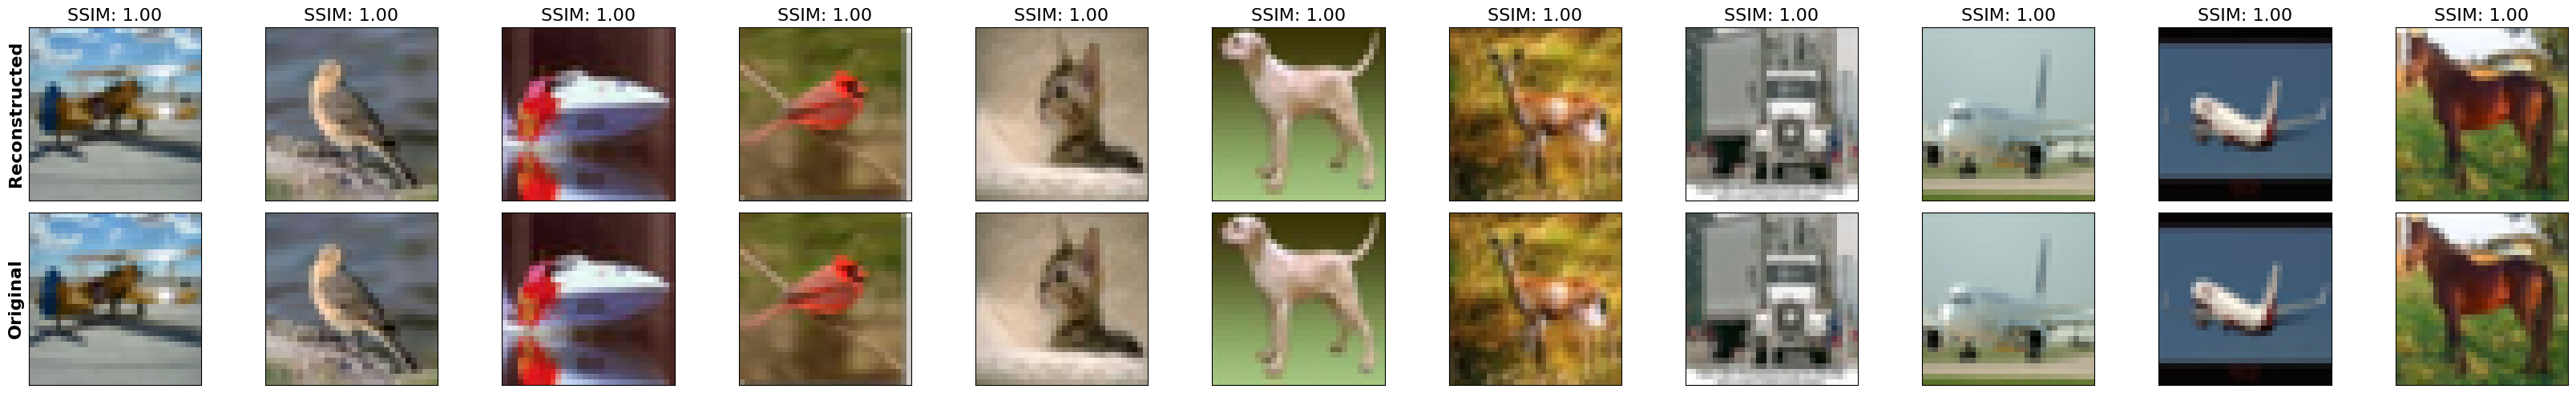
\includegraphics[width=1\linewidth]{assets/chapter_4/cifar/cifar_vgia_rec.png}
    \caption{VGIA reconstruction examples on a batch of $B=2048$ images from CIFAR10.}
    \label{fig:cifar10_example}
\end{figure}

\begin{figure}
    \centering
    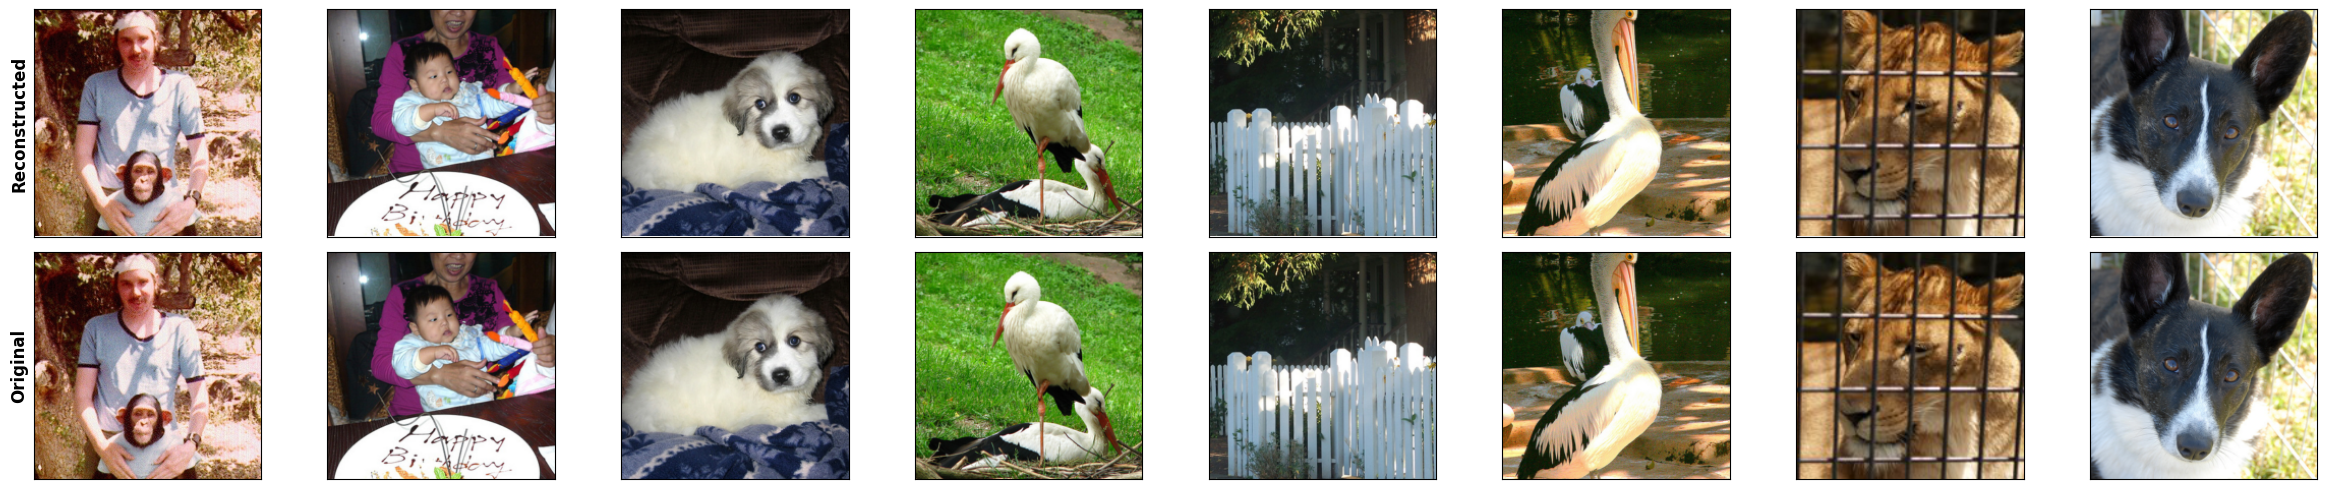
\includegraphics[width=1\linewidth]{assets/chapter_4/imagenet/rec_examples.png}
    \caption{VGIA reconstruction examples on a batch of $B=1024$ images from ImageNet.}
    \label{fig:imagenet_example}
\end{figure}


\begin{table}[h]
\centering
\small
\caption{First 5 features from HARUS reconstructed samples from a batch of $B=2048$ records.}
\begin{tabular}{llrrrrr}
\toprule
Example & Sample &
\texttt{tBody-mean-X} &
\texttt{tBody-mean-Y} &
\texttt{tBody-mean-Z} &
\texttt{tBody-std-X} &
\texttt{tBody-std-Y} \\
\midrule
1 & Rec. & 0.62 & -0.0081 & -0.066 &  0.79 &  0.42 \\
1 & True      & 0.62 & -0.0081 & -0.066 &  0.79 &  0.42 \\
\midrule
2 & Rec. & 0.27 & -0.032  & -0.13  & -0.28 & -0.12 \\
2 & True      & 0.27 & -0.032  & -0.13  & -0.28 & -0.12 \\
\midrule
3 & Rec. & 0.33 & -0.014  & -0.075 &  0.65 &  0.53 \\
3 & True      & 0.33 & -0.014  & -0.075 &  0.65 &  0.53 \\
\midrule
4 & Rec. & 0.25 & -0.026  & -0.21  &  0.66 &  0.55 \\
4 & True      & 0.25 & -0.026  & -0.21  &  0.66 &  0.55 \\
\bottomrule
\end{tabular}
\label{tab:harus-reconstructed-originals}
\end{table}

\begin{table}[h]
\centering
\caption{Reconstruction examples from a batch of 2048 samples of the KCH dataset. The table shows 8 of the 18 features of the dataset.}

\small
\begin{tabular}{llrrrrrrrr}
\toprule
Example & Sample & Bedrooms & Bathrooms & Sqft living & Condition & Grade & Sqft above & Sqft basement & Year built \\
\midrule
1 & Rec. & 6 & 4.75 & 5770 & 3 & 12 & 4500 & 1270 & 1998 \\
1 & True      & 6 & 4.75 & 5770 & 3 & 12 & 4500 & 1270 & 1998 \\
\midrule
2 & Rec. & 4 & 2.50 & 3350 & 3 & 10 & 1760 & 1590 & 1995 \\
2 & True      & 4 & 2.50 & 3350 & 3 & 10 & 1760 & 1590 & 1995 \\
\midrule
3 & Rec. & 2 & 1.75 & 2260 & 3 & 9  & 1890 & 370  & 2005 \\
3 & True      & 2 & 1.75 & 2260 & 3 & 9  & 1890 & 370  & 2005 \\
\midrule
4 & Rec. & 5 & 2.50 & 3490 & 4 & 9  & 1840 & 1650 & 1958 \\
4 & True      & 5 & 2.50 & 3490 & 4 & 9  & 1840 & 1650 & 1958 \\
\bottomrule
\end{tabular}
\label{tab:king-county-reconstructed-originals}
\end{table}
